113. \begin{figure}[ht!]
\center{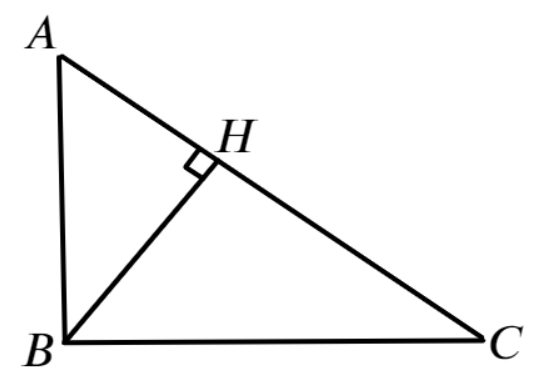
\includegraphics[scale=0.35]{g8-111.png}}
\end{figure}\\
Найдём $\angle A=90^\circ-60^\circ=30^\circ,$ тогда $\angle C=90^\circ-30^\circ=60^\circ,\ \angle CBH=90^\circ-60^\circ=30^\circ.$ По теореме о прямоугольном треугольнике с углом в $30^\circ$ для треугольников $CBH$ и $ABC$ имеем соотношения $BC=2CH=8,\ AC=2BC=16.$ Тогда $AH=AC-CH=16-4=12.$\\
